
%===================================
%===================================
\section{Benchmark}
\label{sec:Benchmark}

En esta sección se presentas los resultados del benchmark realizado sobre las dos maquinas descritas anteriormente. Para este benchmark se usó Geeekbench 6.4.0, el cual se encargó de medir el rendimiento de ambas máquinas. Los resultados se pueden ver en los siguientes enlaces:
\begin{itemize}
    \item \url{https://browser.geekbench.com/v6/cpu/17699747} (Máquina 1)
    \item \url{https://browser.geekbench.com/v6/cpu/17693088} (Máquina 2)
\end{itemize}

\begin{figure}[H]
   \centering
   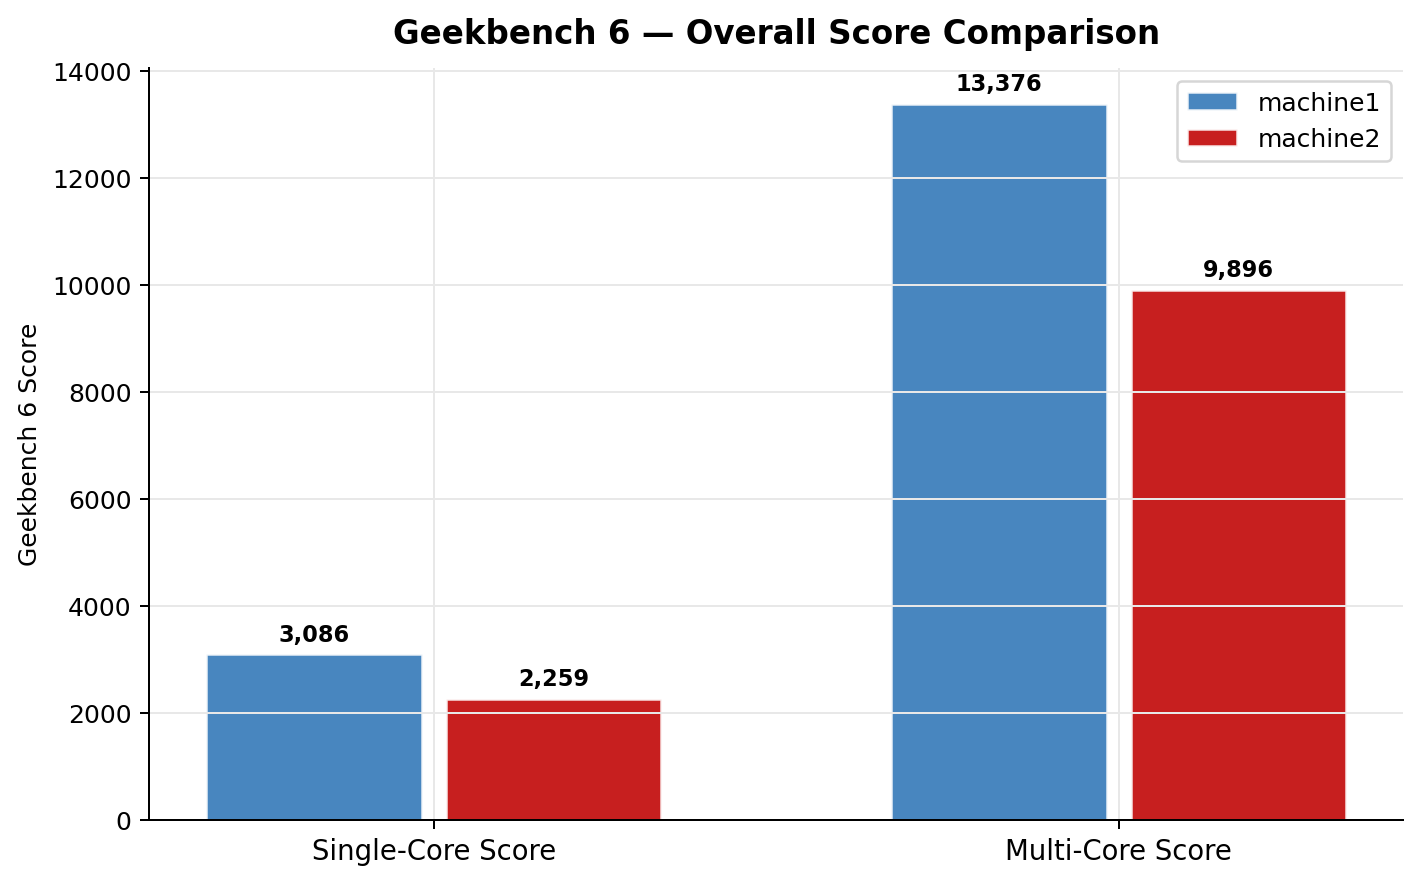
\includegraphics[width=1\textwidth]{images/benchmark/overall_scores.png}
   \caption{Score general de rendimiento para ambas máquinas}
\end{figure}

\begin{landscape}

\begin{figure}[H]
   \centering
   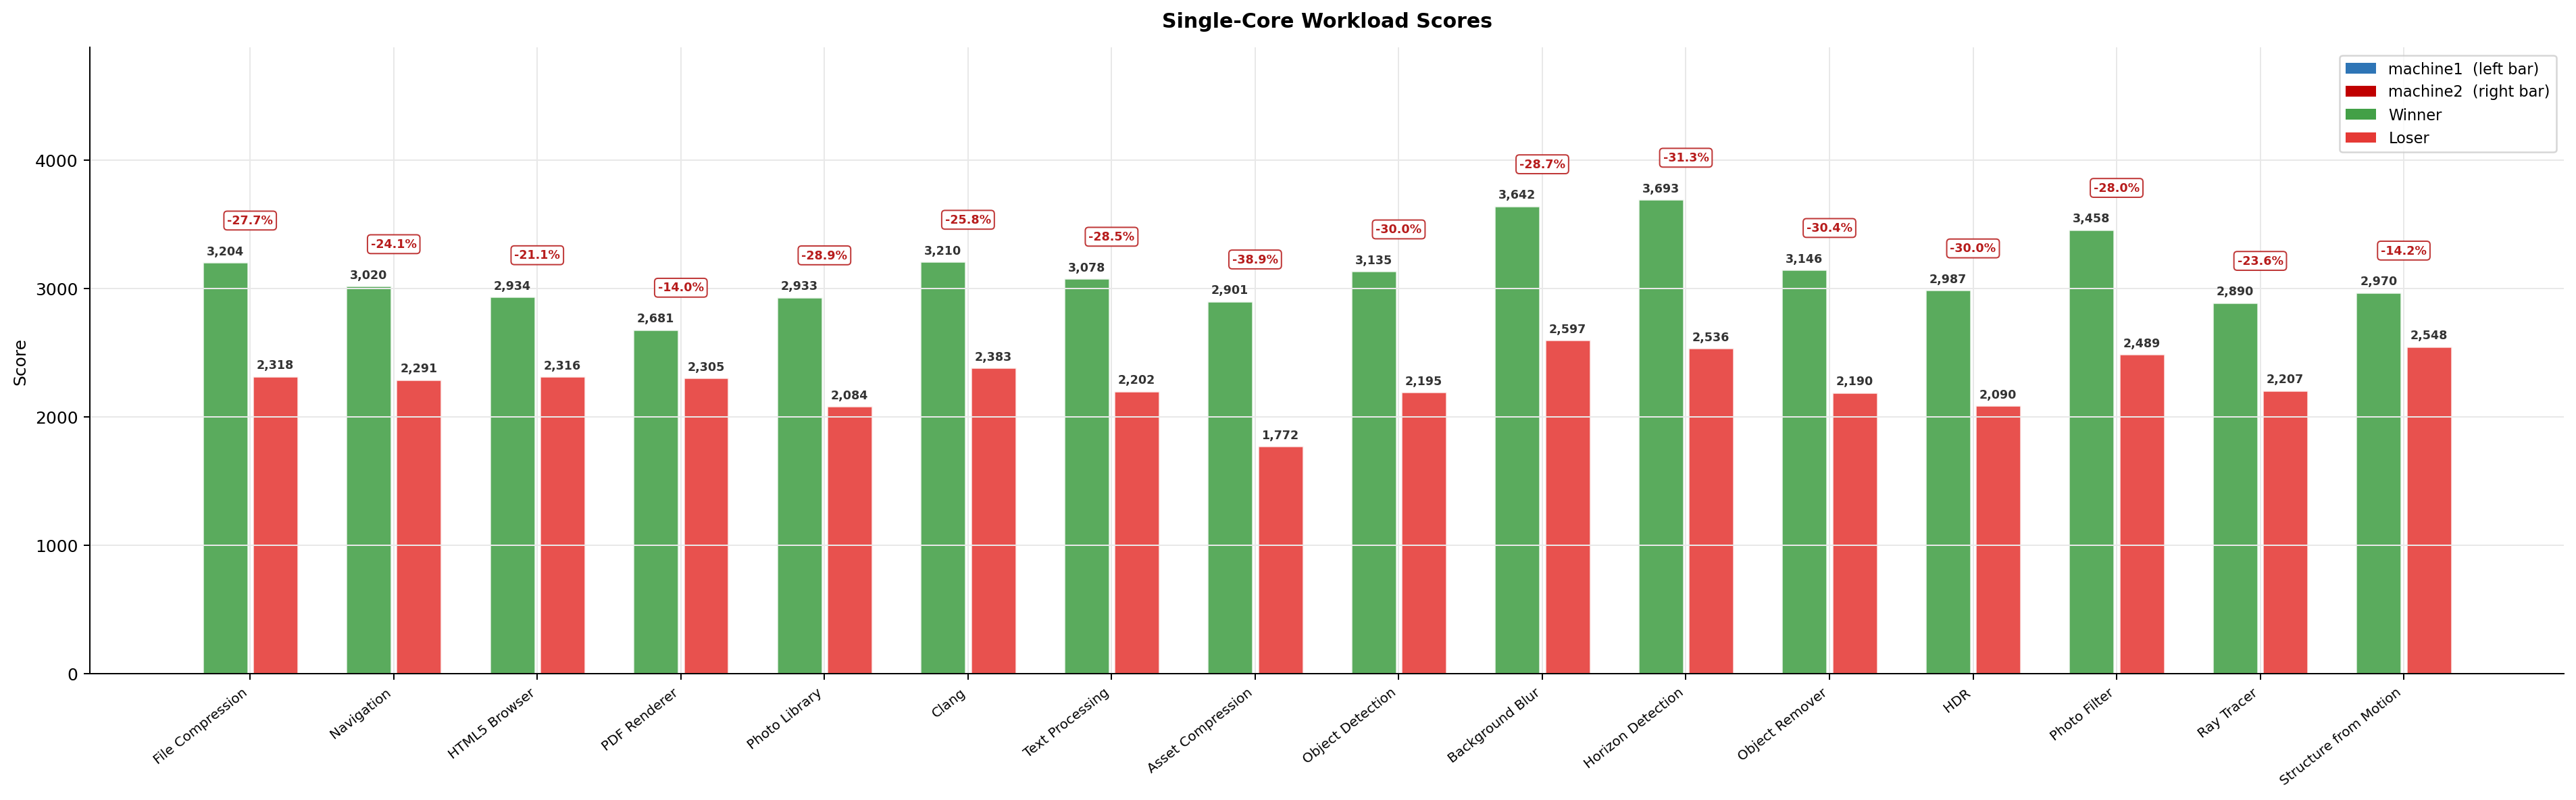
\includegraphics[width=1.3\textwidth]{images/benchmark/workloads_single.png}
   \caption{Rendimiento en single-core para ambas máquinas}
\end{figure}

\begin{figure}[H]
   \centering
   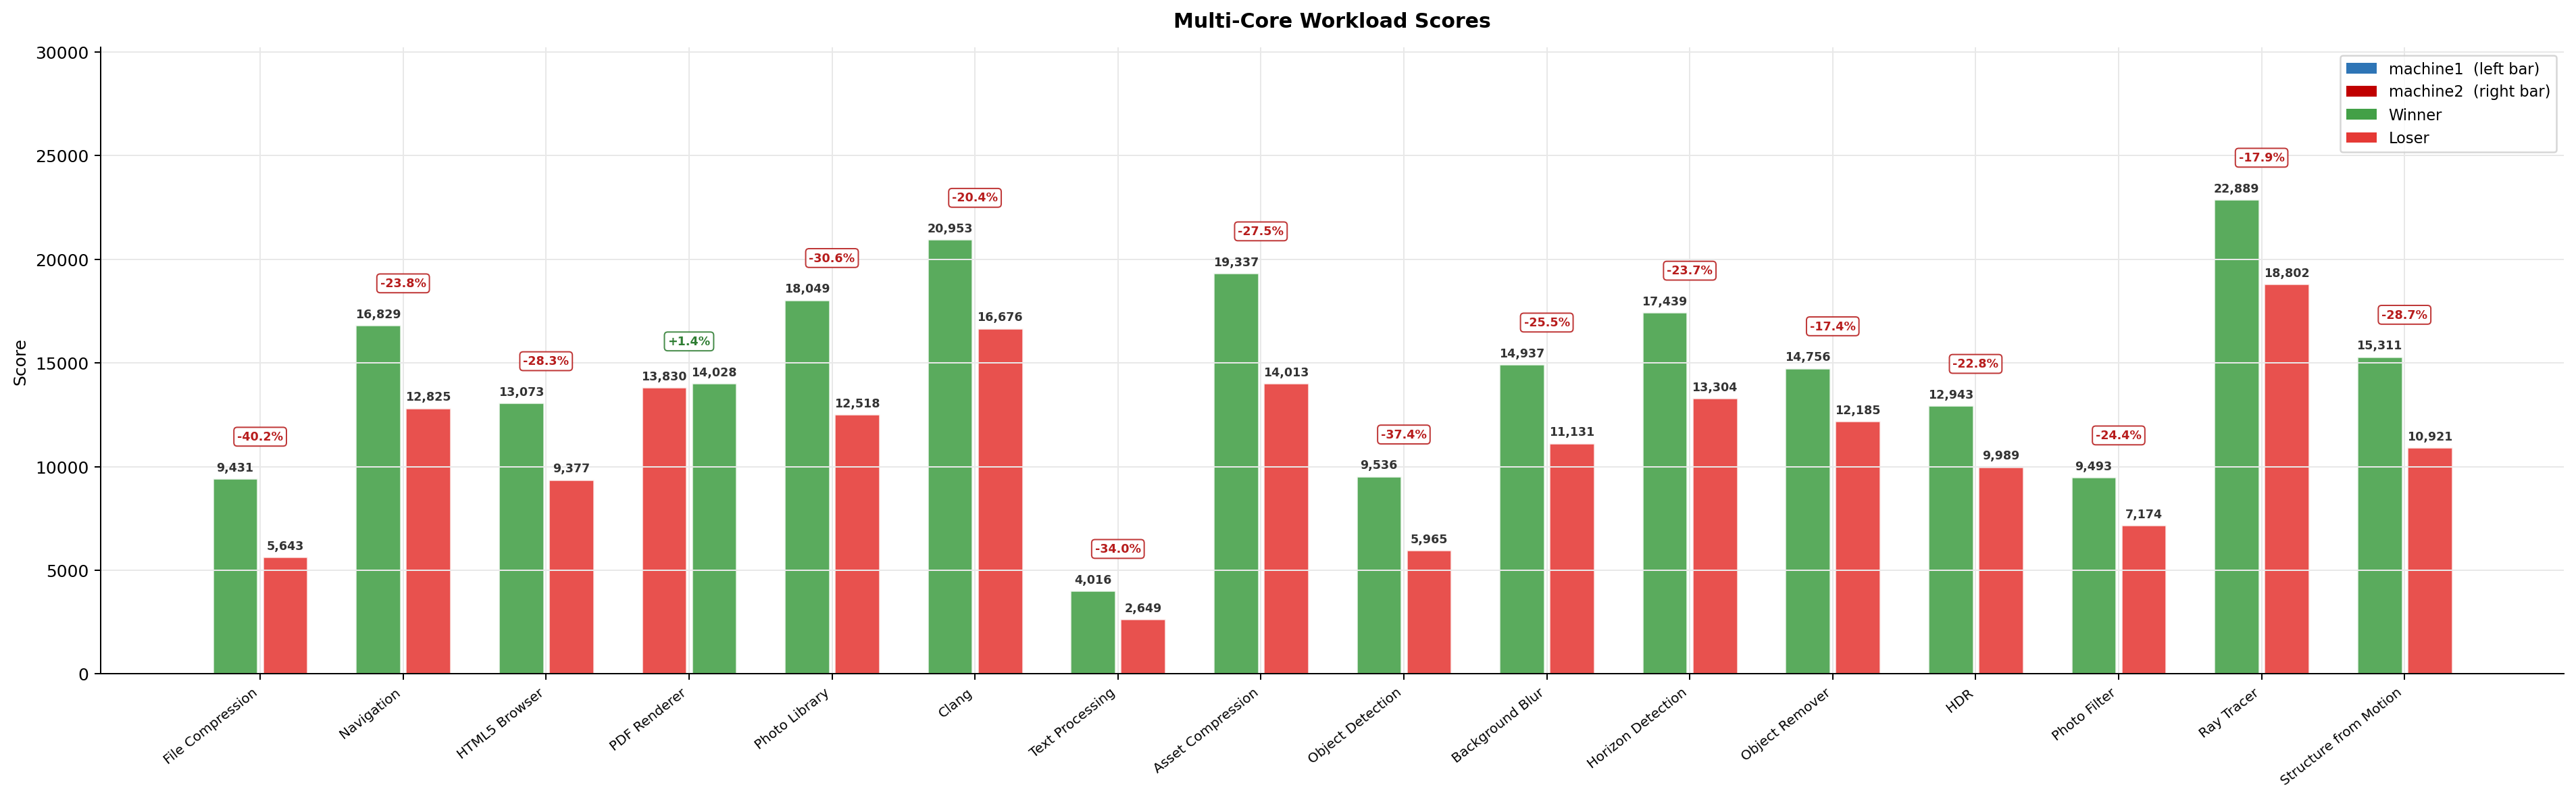
\includegraphics[width=1.3\textwidth]{images/benchmark/workloads_multi.png}
   \caption{Rendimiento en multi-core para ambas máquinas}
\end{figure}

\end{landscape}

\subsection{Descripción de los Sistemas Evaluados}

Los experimentos fueron ejecutados sobre dos plataformas de cómputo con características arquitectónicas distintas. La primera máquina corresponde a un sistema de escritorio equipado con un procesador AMD Ryzen 5 7600X, basado en la microarquitectura Zen 4 (Family 25, Model 97, Stepping 2), con 6 núcleos físicos y 12 hilos de ejecución, operando a una frecuencia observada de 5.46 GHz bajo carga sostenida. Esta plataforma cuenta con 30.23 GB de memoria RAM y está montada sobre una tarjeta madre MSI PRO B650-S WIFI (chipset AMD B650), ejecutando Arch Linux como sistema operativo. La segunda máquina corresponde a un sistema portátil HP Victus 16, equipado con un procesador Intel Core i7-11800H, basado en la microarquitectura Tiger Lake-H (Family 6, Model 141, Stepping 1), con 8 núcleos físicos y 16 hilos de ejecución, operando a una frecuencia observada de 4.60 GHz. Esta plataforma dispone de 15.26 GB de memoria RAM y ejecuta Debian GNU/Linux 12 (Bookworm). Ambos sistemas soportan el conjunto de instrucciones AVX2, AVX-512 y VNNI, y fueron evaluados utilizando Geekbench 6.4.0 para Linux en su modalidad AVX2.

\subsection{Resultados de Rendimiento}

La evaluación de rendimiento mediante Geekbench 6.4.0 revela una ventaja sostenida del sistema desktop AMD Ryzen 5 7600X sobre el sistema portátil Intel Core i7-11800H en la totalidad de las métricas analizadas. En rendimiento de núcleo único, el Ryzen 5 7600X obtuvo una puntuación de 3086 frente a 2259 del i7-11800H, representando una ventaja del 36.6\% que refleja directamente la superioridad IPC de la microarquitectura Zen 4 respecto a Tiger Lake-H. En rendimiento multi-núcleo, el Ryzen 5 7600X alcanzó 13376 puntos frente a 9896 del i7-11800H, una diferencia del 35.2\%, resultado notable considerando que el procesador Intel dispone de dos núcleos físicos adicionales.

A nivel de subtests, el subtest de compresión de activos presentó la mayor brecha en núcleo único con un 63.7\% de ventaja para el Ryzen, atribuible al mayor aprovechamiento de instrucciones SIMD vectoriales. Por su parte, el subtest de procesamiento de texto exhibió el escalado multi-núcleo más bajo en ambas plataformas, 1.30x para el Ryzen y 1.20x para el Intel respecto al score de núcleo único, evidenciando dependencias seriales inherentes a esta carga de trabajo que limitan el beneficio del paralelismo. El subtest de trazado de rayos presentó el mayor ratio de escalado en ambos sistemas (aproximadamente 8x), consistente con su naturaleza paralela. Cabe señalar que las diferencias en configuración de memoria, política de energía y entorno térmico entre ambas plataformas constituyen variables de confusión que deben considerarse al interpretar los resultados comparativos.